\section{Исследовательский раздел}

\subsection{Работа сервера}

На рисунке \ref{fig:200get} показан пример GET запроса.

\begin{figure}[H]
	\centering
	\includegraphics[width=0.9\textwidth]{inc/200\_get.png}
	\caption{GET запрос}
	\label{fig:200get}
\end{figure}

На рисунке \ref{fig:200head} показан пример HEAD запроса.

\begin{figure}[H]
	\centering
	\includegraphics[width=0.9\textwidth]{inc/200\_head.png}
	\caption{HEAD запрос}
	\label{fig:200head}
\end{figure}

На рисунке \ref{fig:403} показана проверка выхода за /root директорию.

\begin{figure}[H]
	\centering
	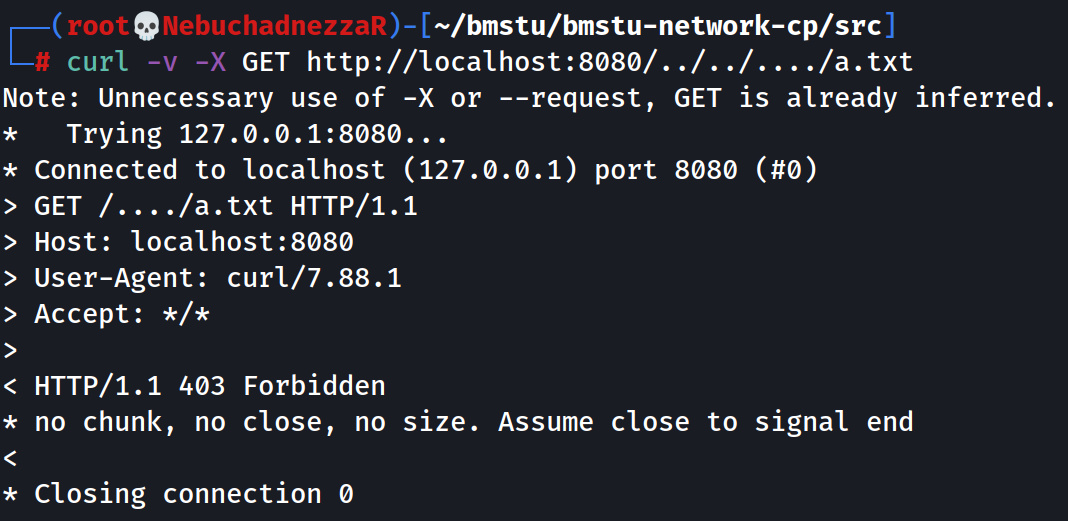
\includegraphics[width=0.9\textwidth]{inc/403.png}
	\caption{Проверка выхода за /root директорию}
	\label{fig:403}
\end{figure}

На рисунке \ref{fig:404} показан пример запроса несуществующего файла.

\begin{figure}[H]
	\centering
	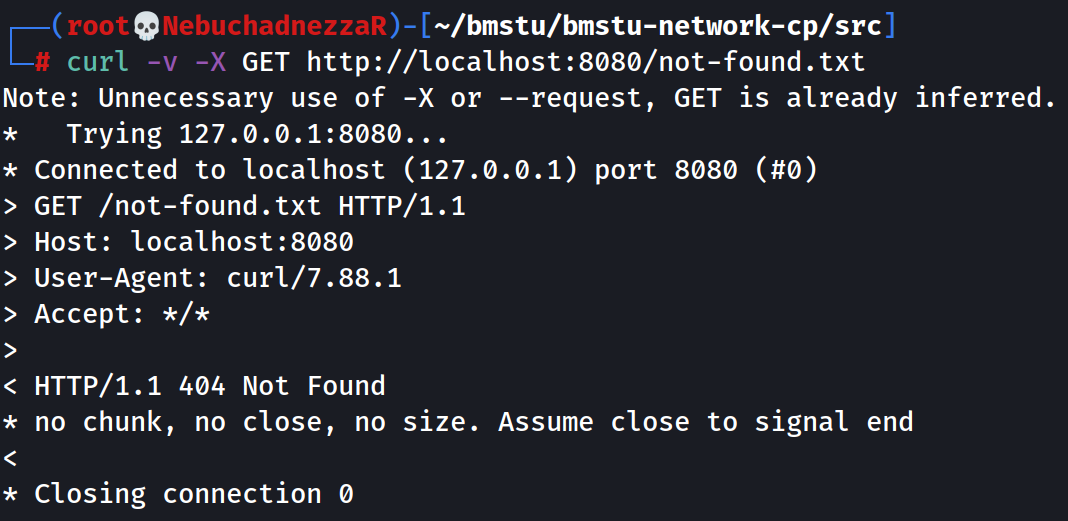
\includegraphics[width=0.9\textwidth]{inc/404.png}
	\caption{Пример запроса несуществующего файла}
	\label{fig:404}
\end{figure}

На рисунке \ref{fig:log} показан пример записи лога.

\begin{figure}[H]
	\centering
	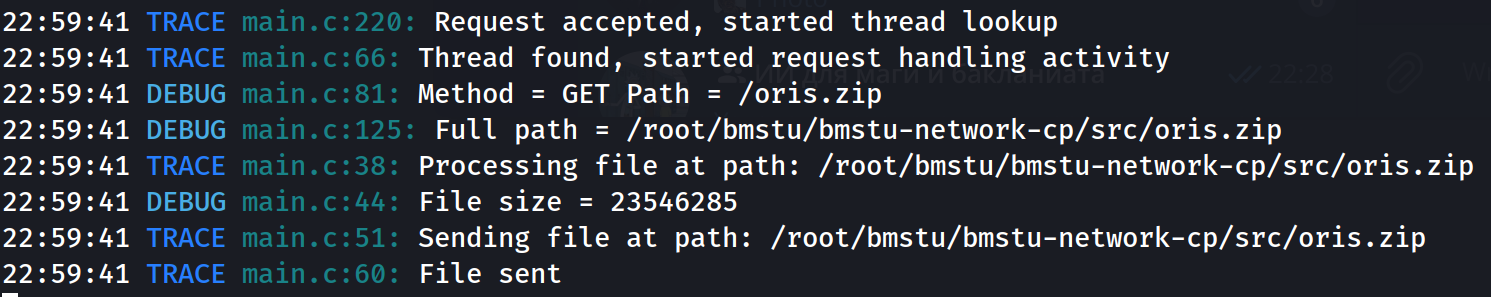
\includegraphics[width=0.9\textwidth]{inc/log.png}
	\caption{Пример записи лога}
	\label{fig:log}
\end{figure}

На рисунке \ref{fig:large_file} показана обработка большого файла.

\begin{figure}[H]
	\centering
	\includegraphics[width=0.9\textwidth]{inc/large\_file.png}
	\caption{Обработка большого файла}
	\label{fig:large_file}
\end{figure}

\subsection{Нагрузочное тестирование}

Нагрузочное тестирование проводилось с помощью ApacheBenchmark, 1000 запросов файла 23Мб в 8 потоков. В качестве альтернативы был настроен сервер nginx. Результаты нагрузочного тестирования представлены в таблице \ref{tab:bench}.

\begin{table}[h]
	\begin{center}
		\caption{Результат нагрузочного тестирования}
		\label{tab:bench}
		\begin{tabular}{|c|c|c|c|c|}
			\hline
			Сервер & Время & Запрос/с & Среднее время запроса & Объём передачи\\
			\hline
			nginx & 7.236с & 138.20 & 7.236мс & 3.03Гб/с \\ \hline
			TP+PS & 5.611с & 178.21 & 5.611мс & 3.9Гб/с \\ \hline
		\end{tabular}
	\end{center}
\end{table}


\clearpage